
%
%  $Description: Author guidelines and sample document in LaTeX 2.09$ 
%
%  $Author: ienne $
%  $Date: 1995/09/15 15:20:59 $
%  $Revision: 1.4 $
%

\documentclass{sig-alternate}
\usepackage{dblfloatfix}
\usepackage{epsfig}
\usepackage{listings}
\usepackage{subfigure}
\usepackage{url}

%------------------------------------------------------------------------- 
% Begin patch area for accents in 'Author Block' area - may be needed by
% some authors / but not all
\DeclareFixedFont{\auacc}{OT1}{phv}{m}{n}{12}   % Needed for "Author Block" accents - Patch by Gerry 3/21/07
\DeclareFixedFont{\afacc}{OT1}{phv}{m}{n}{10}   % Needed for "Author Block" accents in the affiliation/address line - Patch by Gerry 3/21/07
%------------------------------------------------------------------------- 

\begin{document}

\conferenceinfo{HPDC'07,} {June 25--29, 2007, Monterey, California, USA.}
\CopyrightYear{2007}
\crdata{978-1-59593-673-8/07/0006}

\title{User-level Grid Monitoring with Inca 2}

\numberofauthors{1}

\author{
\alignauthor
Shava Smallen, Kate Ericson, Jim Hayes, Catherine Olschanowsky \\
\affaddr{San Diego Supercomputer Center} \\ 
\affaddr{University of California, San Diego} \\ 
\affaddr{9500 Gilman Drive, La Jolla, CA 92093-0505, USA}\\ 
\email{\{ssmallen,kericson,jhayes,cmills\}@sdsc.edu}\\
}

\maketitle

%1.  Motivate and differentiate the Grid monitoring Inca does
%2. Describe Inca 2 design and its benefits
%3. Illustrate that Inca 2 design is mature and being used in production by
%several Grids
%4. Be different from Inca 1 paper

\begin{abstract}
The primary goal in the creation of Grids is to provide unified and coherent
access to distributed computing, data storage and analysis, instruments, and
other resources to advance scientific exploration.  Grids combine multiple
complex and interdependent systems that span several administrative domains.
This complexity poses challenges for both the administrators who build and
maintain the Grid resources and the scientists who use them.  While other Grid
monitoring tools provide system-level information on the utilization of Grid
resources, the Inca system provides user-level Grid monitoring with periodic,
automated user-level testing of the software and services required to support
Grid operation.  Inca can be used by Grid operators, system administrators,
and application users to identify, analyze, and troubleshoot user-level Grid
failures, thereby improving Grid stability.  In this paper, we describe the new
features of our current Inca release, Inca 2.  We then describe the
architecture of the Inca 2 system, in addition to use cases that describe two
Inca 2 deployments in production environments.  
\end{abstract}

%------------------------------------------------------------------------- 

% A category with the (minimum) three required fields
\category{C.4}{Performance Of Systems}{Performance attributes, Reliability,
availability, and serviceability}

\terms{Performance, Reliability, Verification}

\keywords{User-level Grid monitoring, Grid monitoring, TeraGrid}

%------------------------------------------------------------------------- 
\section{Introduction}
\label{intro}

% Standard "Grids are good" intro paragraph.  But are complex.  
Grid systems provide unified and coherent access to distributed computing,
data storage and analysis, instruments, and other resources.  These systems
require the careful coordination of software packages, services, and
configurations across multiple, potentially heterogeneous, resources.  For
example, the TeraGrid project~\cite{teragrid} manages the coordination of
software and services by deploying and monitoring a common user environment
across distributed, heterogeneous resources. 
TeraGrid's software and services uniformity simplifies access to its
resources, which consist of more than 102 teraflops of compute capability and
more than 15 petabytes of online storage, all interconnected by a network that
can transfer a terabyte of data in under 10 minutes.  

% Complex means they are difficult to provide and maintain. Describe the
% stakeholders.   Monitoring is needed.
Providing and maintaining a stable infrastructure for these complex 
Grid systems poses challenges for both administrators who build and
maintain Grid resources and scientists who use them.  System
administration is distributed across multiple administrative domains 
requiring a significant amount of coordination.  This is typically performed by
a group of Grid administrators or operators who consider local site policies and
resource heterogeneity
and decide when software (including updates and patches) should be deployed to
resources and how it should be configured.  
Each site's system administrators, who are not necessarily Grid
experts, are then responsible for providing the required Grid software
components and services for their resource and debugging any problems that
arise.  Well-defined requirements and good communication are required in this
model; otherwise, inconsistencies arise between the resources that either
inconvenience the user or prevent them from using a particular resource
altogether.  Periodic failures that occur in Grid services due to network or
system failures, software misconfiguration, or software bugs also present a
challenge.  Grid monitoring can be used to detect such problems, leading to a
more stable and dependable Grid infrastructure.

% What types of Grid monitoring are around and what the limitations are
One approach to monitoring Grids, used by tools such as
MonALISA~\cite{monalisa} and GridICE~\cite{gridice}, is to aggregate and
display data from existing cluster or system administrator monitoring tools
such as Ganglia~\cite{ganglia}, CluMon~\cite{clumon}, or
Nagios~\cite{nagios}.  This provides a centralized, systems-level view of Grid
resources where low-level host statistics and queue information can be
examined.  This type of monitoring information is useful for showing the
utilization of Grid resources, but it does not provide the type of
high-level monitoring needed to detect user problems, such as incompatible
software components, within the Grid infrastructure.  Industry monitoring
tools are also available such as IBM Tivoli Monitoring~\cite{tivoli} and
Microsoft Operations Manager~\cite{mom}, which monitor and manage large
networks of services.  However, these tools depend on proprietary software and
are targeted to a single administrative domain, which is unsuitable for Grid
systems that span multiple administrative domains.

% What user-level monitoring provides and why we think it is good
User-level Grid monitoring provides Grid infrastructure testing and performance measurement 
from a generic, impartial user's perspective.  The goal of user-level monitoring is 
to detect and fix Grid infrastructure problems before users notice them by
notifying site system administrators and providing them with the error details -- 
user complaints should not be the first indication of Grid failures.  
In our view, successful user-level Grid monitoring needs to include
these features:

\begin{itemize}

\item Runs from a standard user
account in order to reflect regular user experiences.  It is important not to execute from a system administrator's account,
which may have special privileges and use custom shell initialization files.

\item Executes with a standard user GSI credential mapped to a standard user
account when tests or performance measurements require authentication to Grid
services.

\item Emulates a regular user by using tests and performance measurements
created and configured based on user
documentation, rather than on system administrator knowledge (of hostnames,
ports, pathnames, etc.).  In cases where documentation and tests are developed
simultaneously during pre-production, test development should
be closely coordinated with the documentation as it is written.

\item Centrally manages the configuration of user-level tests or performance
measurements in order to ensure consistent testing across resources.

\item Easily updates and maintains user-level tests and performance
measurements.  This is important because tests and measurements are often
updated when Grid infrastructure changes.
Also, multiple iterations of test development are often required to
determine whether a detected test failure stems from a faulty test,
incomplete user documentation, or a failed Grid resource.  

\item Provides a representative indication of Grid status by testing
documented user commands and individual Grid software components.  

\item Automates the periodic execution of user-level tests or performance
measurements to understand Grid behavior over time.

\item Executes locally on Grid resources to verify user accessible Grid access
points.  Executes from each resource to every other resource (all-to-all) to
detect site-to-site configuration errors such as authentication problems.

\end{itemize}

% Inca 1~\cite{inca1} first addressed user-level Grid monitoring but had
% limitations.  We learned lessons from our TeraGrid deployment and
% developed Inca 2.

\noindent In 2003 SDSC, in partnership with TeraGrid, began developing Inca
1~\cite{inca1} to implement a user-level Grid monitoring system that provided
these features.  At that time, the only available user-level Grid
monitoring tools were the NCSA TestGrid script~\cite{ncsa-test} and
Grid Integration Test Script (GITS)~\cite{gits}, both of which ran a fixed number of Grid tests and formatted
results in HTML.  Although these tools were easy to install and produced
useful information, they showed the view of the Grid from a single
resource, lacked automation, and were not easily extensible.  Inca 1 provided
the means to verify that the common user environment was deployed consistently
across all TeraGrid resources and to monitor its status.

The initial
version of Inca was implemented as a client-server architecture.  It provided
data collection, data storage (accessible from a Web services interface and with 
limited archiving capabilities), and data display though Web status
pages.  Inca 1 was first deployed to TeraGrid in mid 2003 and released in late
2003. Running Inca 1 for a year and a half on TeraGrid taught 
valuable lessons that have been incorporated into the design of Inca 2, our
current release.  Inca 2
contains a number of substantial improvements over Inca 1 with respect to
security, installation and maintenance, and storage capabilities.  Inca 2 has
been running on TeraGrid since November 2006, and a production
version of the software was released in February 2007.  Currently, seven other Grids in the
U.S., Europe, and Australia use Inca 2.  

% This motivated our development of a new version of Inca.
In the next section, we describe the design goals and features of Inca 2. 
We then describe the Inca 2 architecture and how it can be used to provide
user-level Grid monitoring.  In Section~\ref{usecases}, we describe two 
uses of Inca 2 for Grid software environment verification and benchmarking.  
Finally, we describe some future work and summarize the paper.

%------------------------------------------------------------------------- 
\section{Inca 2 Features}
  
\begin{figure*}[tbp]
  \centering
  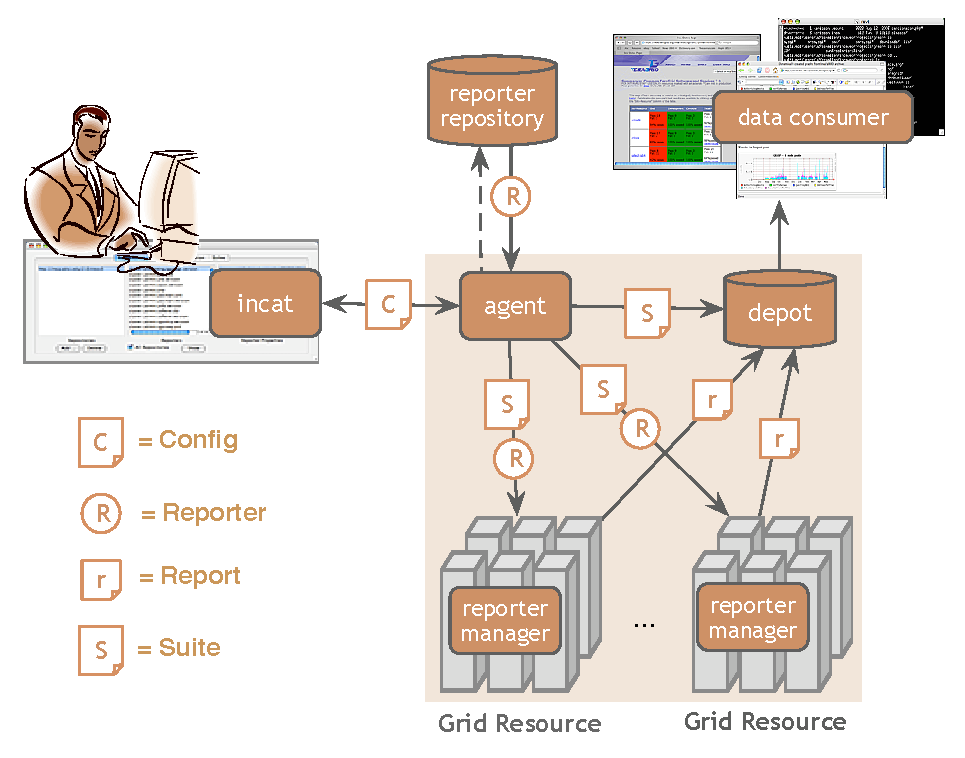
\includegraphics[width=.6\textwidth]{arch.eps}
  \caption{\label{arch_fig} Inca architecture.}
\end{figure*}

% Implements user-level Grid monitoring and who it benefits
Inca 2 is a system that provides user-level monitoring of Grid functionality
and performance.  It was designed to be
general, flexible, scalable, and secure, in addition to being easy to deploy
and maintain.  Inca benefits Grid operators who oversee the day-to-day
operation of a Grid, system administrators who provide and manage resources,
and users who run applications on a Grid.  Besides implementing the features
described in Section~\ref{intro}, Inca 2 has additional features
listed below.  A '*' after a feature description indicates it is a new
feature of Inca 2; other items note improvements to Inca 1 features.  The 
Inca system:

\begin{enumerate}

\item Collects a wide variety of user-level monitoring results (e.g., simple
test data to more complex performance benchmark output).  

\item Captures the context of a test or benchmark as it executes (e.g.,
executable name, inputs, source host, etc.) so that system administrators have
enough information to understand the result and can troubleshoot system
problems without having to know the internals of Inca. 

\item Eases the process of writing tests or benchmarks and deploying them into
Inca installations. 

\item Provides means for sharing tests and benchmarks between Inca users. *

\item Easily adapts to new resources and monitoring requirements in order to
facilitate maintenance of a running Inca deployment. 

\item Stores and archives monitoring results (especially any error messages) 
in order to understand the behavior of a Grid over time. The results
are available through a flexible querying interface.

\item Securely manages short-term proxies for testing of Grid services using
MyProxy~\cite{myproxy}. *

\item Measures the system impact of tests and benchmarks executing on
the monitored resources in order to tune their execution frequency and
reduce the impact on resources as needed. *

\end{enumerate}

\noindent The following section describes how the Inca architecture implements
these features.

%------------------------------------------------------------------------- 
\section{Inca 2 Architecture}

% overview description of components
Figure~\ref{arch_fig} shows the architecture of Inca 2, which
incorporates three core
components (highlighted box) -- the agent, depot, and reporter manager.
The \textit{agent} and \textit{reporter managers} coordinate the execution of
tests and performance measurements on the Grid resources and the
\textit{depot} stores and archives the results.  The inputs to Inca 2 are one
or more \textit{reporter repositories} that contain user-level tests and
benchmarks, called \textit{reporters}, and a configuration file describing how
to execute them on the Grid resources.  This configuration is normally created
using an administration GUI tool
called \textit{incat} (Inca Administration Tool).  The output or results
collected from the resources are queried by the \textit{data consumer} and
displayed to users.  The following steps describe how an Inca administrator
would deploy user-level tests and/or performance measurements to their
resources.

\begin{enumerate}

\item The Inca
administrator either writes reporters to monitor the user-level functionality
and performance of their Grid or uses existing
reporters in a published repository.

\item The Inca administrator creates a deployment configuration file that
describes the user-level monitoring for their Grid using incat and submits it
to the agent.

\item The agent fetches reporters from the reporter repository, creates a
reporter manager on each resource, and sends the reporters and instructions for
executing them to each reporter manager.

\item Each reporter manager executes reporters according to its schedule and
sends data to the depot.

\item Data consumers display collected data by querying the depot.
\end{enumerate}

\noindent The following subsections describe the Inca components in more
detail, using the order of the steps above.

\subsection{Reporters}

\lstset{
  basicstyle=\scriptsize\fontfamily{phv}\selectfont, 
  frame=single,
  keywordstyle=\textbf, 
  identifierstyle=, 
  commentstyle=\scriptsize, 
  stringstyle=, 
  numbers=left, 
  numberstyle=\scriptsize,
  stepnumber=2,
  firstnumber=1,
  showstringspaces=false} 
\begin{figure}[tbp]
\lstset{language=Perl} 
\subfigure[]{\lstinputlisting{grid.globus.gramPing}}
\lstset{language=XML,keywordstyle={}} 
\subfigure[]{\lstinputlisting{grid.globus.gramPing.out}}
\caption{\label{pingReporter}(a) An Inca reporter that tests the user-level
availability of a Globus GRAM server and (b) sample of its output.}
\end{figure}

An Inca reporter is an executable program that tests or measures some aspect
of a system or installed software.   Reporter executables are designed to be
easy to produce and can be run outside of the Inca system (e.g., by a system
administrator).  Existing reporters range from a simple Globus~\cite{globus}
GRAM gatekeeper ping test (see Figure~\ref{pingReporter})
to complex Grid application benchmarks~\cite{grasp}.  Reporters must
support certain command line options and produce an XML document, or
\emph{report},
according to the Inca reporter schema.  The goal of the reporter schema is to
accommodate multiple types of data and to capture enough information about the
reporter execution to diagnose any detected failures.  The reporter schema
consists of the following elements: 

\begin{itemize}
\item a set of header tags describing the context of the reporter
execution:  GMT timestamp, hostname, reporter name, reporter version, working
directory, reporter path, and arguments;
\item an optional set of debug or information log tags similar to log4j~\cite{log4j} output;
\item a body containing the results expressed as an XML sequence; and
\item an exit status tag
indicating whether the reporter was able to complete its test or measurement,
and an optional error message.  
\end{itemize} 
\noindent Because the body of a report can be any XML sequence, it enables
reporters to express a wide variety of information.  Today, we have four
standard body schemas to express software version information, software
functionality or service tests results, usage information, and performance
results.  

An extensible set of Perl APIs is provided to handle much of the effort of
writing reporters.  Figure~\ref{pingReporter} shows (a) an Inca reporter that
pings a pre-WS Globus GRAM server and (b) its corresponding output when
executed on a local machine.  The reporter uses two of the Perl APIs:
\linebreak Inca::Reporter::SimpleUnit (a subclass of Inca::Reporter)
\linebreak and
Inca::Reporter::GridProxy.  The Inca::Reporter API provides convenience
functions for handling the required input arguments
(lines~\ref{pingReporter}(a) 12-14 produces lines \ref{pingReporter}(b)
10-31) and printing the Inca-compliant header and exit status XML tags
(lines~\ref{pingReporter}(a) 3-10, 24 produces \ref{pingReporter}(b)
1-9, 43-46).  It also includes some informational and debug logging functions
similar to log4j.  The log output has been very useful to system
administrators, who can view a summary of the test or benchmark that the
reporter performed without reading the reporter source code.  Line
\ref{pingReporter}(a) 15 shows a special log function, loggedCommand, that
executes a system command (using a 30 second timeout) after logging it to the
'system' level of the log XML (producing lines \ref{pingReporter}(b) 32-37).  The subclass
Inca::Reporter::SimpleUnit is the API responsible for printing the simplest
standard reporter body schema that reports software functionality or service
tests results; it handles the printing of the small body XML
(lines~\ref{pingReporter}(b) 39-41).  Finally, the
Inca::Reporter::GridProxy dependency (line~\ref{pingReporter}(a) 11) adds a proxy
dependency to the reporter, telling Inca to download a
short-term proxy before running this reporter (as discussed in
Section~\ref{security}).  Most current reporters use the Perl APIs and consist
of fewer than 30 lines of code.

\subsection{Reporter Repositories}

% What are repositories and their key features
Reporter repositories are collections of reporters, required
packages and libraries (including the Perl APIs described in the previous
section), and a catalog file.  Repository contents are accessible using a URL
and designed to be shared across multiple Inca deployments.  The catalog file,
patterned after APT's Packages.gz~\cite{apt}, allows the user to indicate
reporter dependencies on CPAN modules, tar.gz packages, and other external
sources.  Inca automatically deploys dependencies into a
subdirectory of its installation (see Section~\ref{agent}); this enables
reporters to be deployed to resources with minimal delay.  Each package
specified in the catalog is versioned, allowing Inca to
automatically distribute reporter code updates such as bug fixes.  Because of
this, Inca administrators who maintain repositories need to ensure
that updates to reporters work properly before committing them to a repository.

% We have a lot of reporters ready to be picked 
The Inca team publishes a reporter repository that contains 143 reporters
developed for TeraGrid.  Most reporters are either version
reporters that collect version information from a software package,
unit test reporters that run a more involved
functionality test, or performance benchmark reporters.  The unit and version
reporters cover software such as Grid middleware and tools, compilers, math libraries,
data tools, and visualization tools.  Current performance reporters
measure data transfer and execute Grid benchmarks as described in
Section~\ref{grasp}.

\subsection{Inca administration tool (incat)}

\begin{figure*}[tbp]
  \centering
  \mbox{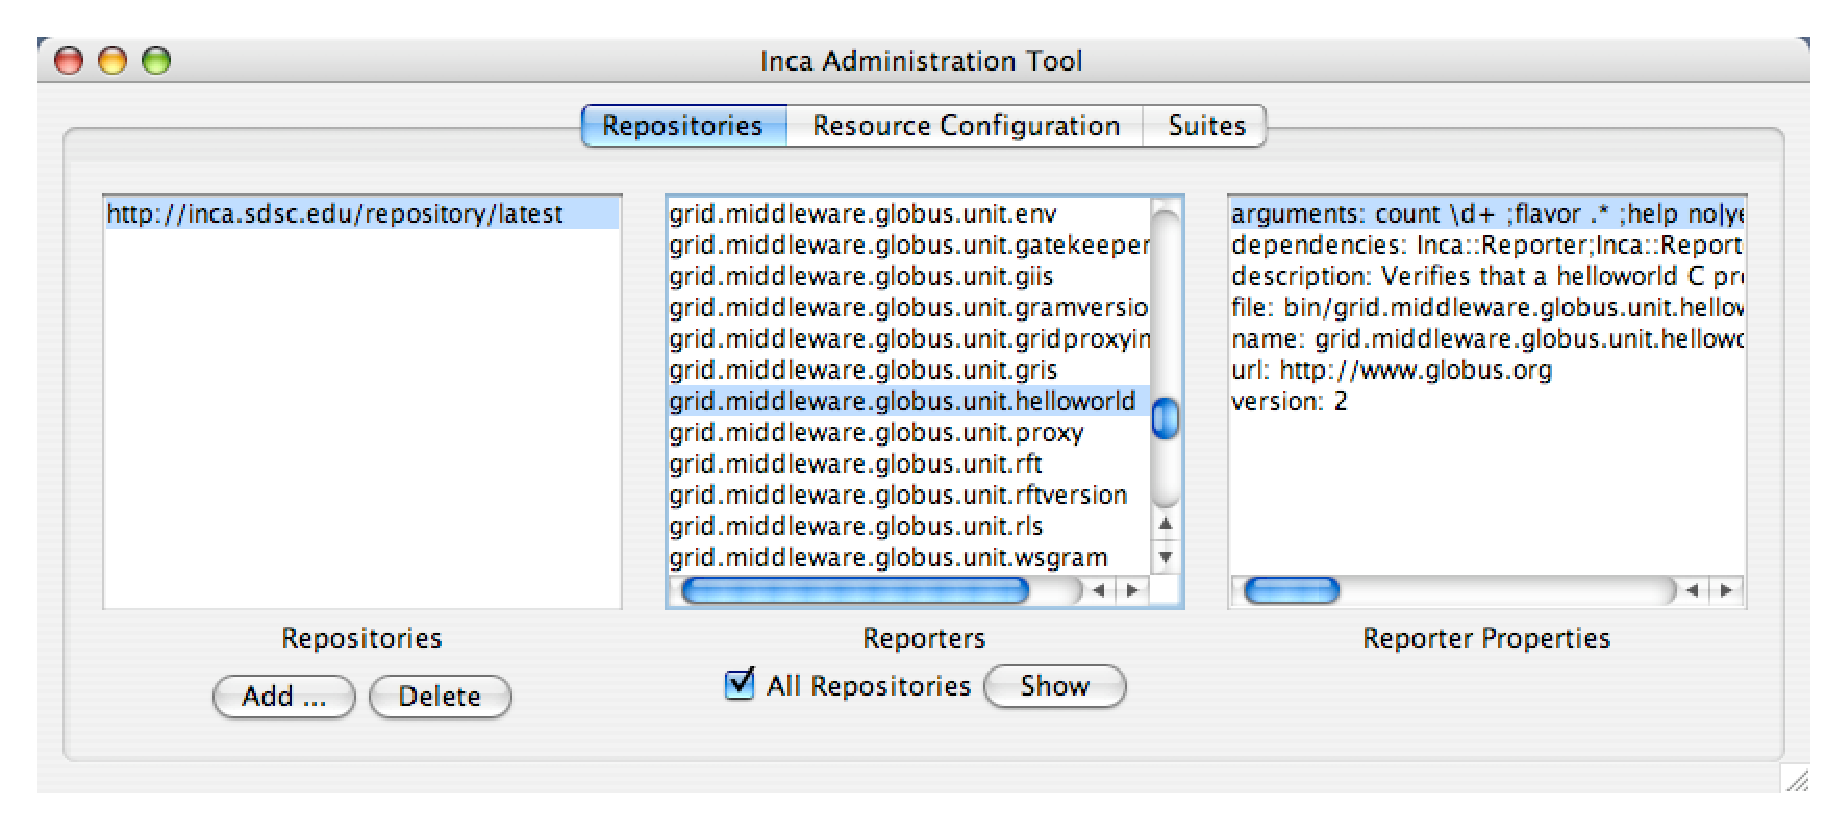
\epsfig{file=incat.eps, width=.9\textwidth}}
  \caption{\label{incat_fig} Screenshot of incat that shows the reporters
  and their attributes available from the reporter repository.}
\end{figure*}

% Incat is interface Inca admin uses to configure reporters to resources
% introduce series here; why suites are important It is designed to make the
% effort of configuring and maintaining 100s series on resources easilty
The Inca administrative tool (incat) is a Java Swing GUI that
Inca administrators use to configure user-level Grid monitoring on their
resources.  Incat allows an Inca administrator to choose which resources to
monitor and which reporters to deploy to those resources.  The configuration
is stored in a XML file and sent to the agent, which handles its implementation
(described in the next section).  The Inca administrator can reload the
configuration to make updates.  Incat provides a number of
conveniences that enable a large number of results to be managed and collected
with a minimum effort.  

To begin reporter configuration, the Inca administrator enters the location of
one more reporter repositories, and incat loads and displays the reporters
available from them (Figure~\ref{incat_fig}).
For each reporter, the Inca administrator can specify the resources to run on,
input arguments, the runtime environment, the frequency of execution, resource
limits, and email notifications.  The sequence of reports that a reporter
produces on a resource when executed with a specific set of input arguments and
runtime environment is known as a \emph{report series} (or \emph{series} for
short).
Thus, the grid.globus.gramPing reporter in Figure~\ref{pingReporter} would
produce one report series when executed with 'blue.ufo.edu' as the host argument and another report series with 'red.ufo.edu'.  A set of related
series can be grouped into \emph{suites} and shared across other Inca
deployments, e.g.,  a Globus suite or a data transfer
performance suite.  Suites can also be useful in determining interoperability
among Grids or whether an application's requirements are being
fulfilled on a Grid.

% Resource information organized to make it easier to maintain
For each monitored resource, an Inca administrator selects an access method
(SSH or Globus) to access the resource and start monitoring there (described
in Sections~\ref{agent} and ~\ref{rm}).  Resources can be aggregated into
groups for reference in the series configuration, facilitating the
process of executing the same series on multiple resources.  Also,
input and runtime environment attributes can be attached to resource groups
for reference in series configuration.
These resource \emph{macros} can have multiple values, in which
case the series will be executed on the resource once for each macro value.
Resource groups and macros ease the process of defining and maintaining
multiple similar series.

\subsection{Agent}
\label{agent}

The Inca agent is a server that implements the configuration specified by the
Inca administrator.  When the agent receives a configuration from incat,
it expands any resource group and macro references to determine
the series to execute on each resource and stores this
information in the depot.  The agent stages and
launches an Inca component, called a reporter manager (described in the
following subsection), on each resource, using either SSH or Globus.  After a
reporter manager contacts its agent, the agent transmits the reporters to
execute, any dependencies, and a suite that contains series
configuration and an execution schedule.  As an Inca administrator makes
updates to the configuration, the agent will push out new reporters and/or
suite changes to each of the affected resources.

The agent regularly pings its reporter managers in order to detect when one has
failed (for example, when a system is taken down for maintenance) and so must
be restarted.  The agent also maintains a local cache of reporters and their
dependencies; it periodically checks repositories
and automatically distributes reporter updates to the reporter managers as
needed.  The agent is implemented using Java. 

\subsection{Reporter Manager}
\label{rm}

The Inca reporter manager is a lightweight process responsible for managing
the schedule and execution of Inca reporters on a single resource. The
reporter manager receives reporter updates and dependencies from the agent
along with requests for reporter scheduling changes.  Running under a regular
user account, the reporter manager executes reporters on-demand or using an
internal cron scheduler and sends reports to the depot for archiving. The
reporter manager monitors reporter system usage 
and enforces limits (e.g., wall clock time, CPU time, memory).
System usage information is sent to the depot with each report. 
The reporter manager is implemented using Perl to allow execution on
a wide variety of UNIX systems.

\subsection{Depot}

The Inca depot server is responsible for storing configuration information and
the data produced by reporters. The depot uses a relational database via
Hibernate~\cite{hibernate}, enabling the use of a variety of database backends.
The depot provides full archiving of reporter output, and the database schema is
tuned to minimize redundant data.  Inca administrators can specify pattern
tests to run on reports as they are received, and the depot will send email
when the results of these tests change.  This provides the administrator
with quick notification of problems as they appear and of the results of
repairs.

Data can be retrieved using SQL queries. Predefined queries exist to return the
latest report instances of a suite, a single report instance, or a report
history.  A Web services interface is also available to provide
unauthenticated query access to data.  The depot is implemented using Java.

\subsection{Data Consumer}

The Inca data consumer is a Web application that queries the Inca depot for
data and displays it in a user-friendly format.  The data consumer is packaged
with Jetty~\cite{jetty} so that Web pages can be served out of the box.  A set
of extensible JSP tags and pages query the Inca depot for data (returned as
XML)
and a set of XSL stylesheets format the data as HTML.  An Inca administrator
can customize the data display, either by modifying the XSL stylesheets or by
writing their own JSP tags and pages.

\subsection{Security}
\label{security}

To provide for security, all Inca components communicate with each other using
SSL, and sensitive information is encrypted before being written to disk.  To
handle reporters that
require a proxy credential to execute, the reporter manager fetches a
short-term proxy from a MyProxy~\cite{myproxy} server (as specified by an Inca
administrator), then destroys the proxy once the reporter has completed.
MyProxy authentication information is fetched from the agent each time a proxy
credential is needed and then cleared from memory.  Generating short-term 
proxies as needed is more secure than maintaining long-term
credentials and is easier to manage.

\vfill\eject 

\subsection{Coordinating Inca Deployments}

% Should illustrate that we've thought about how Inca can scale
\begin{figure*}[tbp]
  \centering
  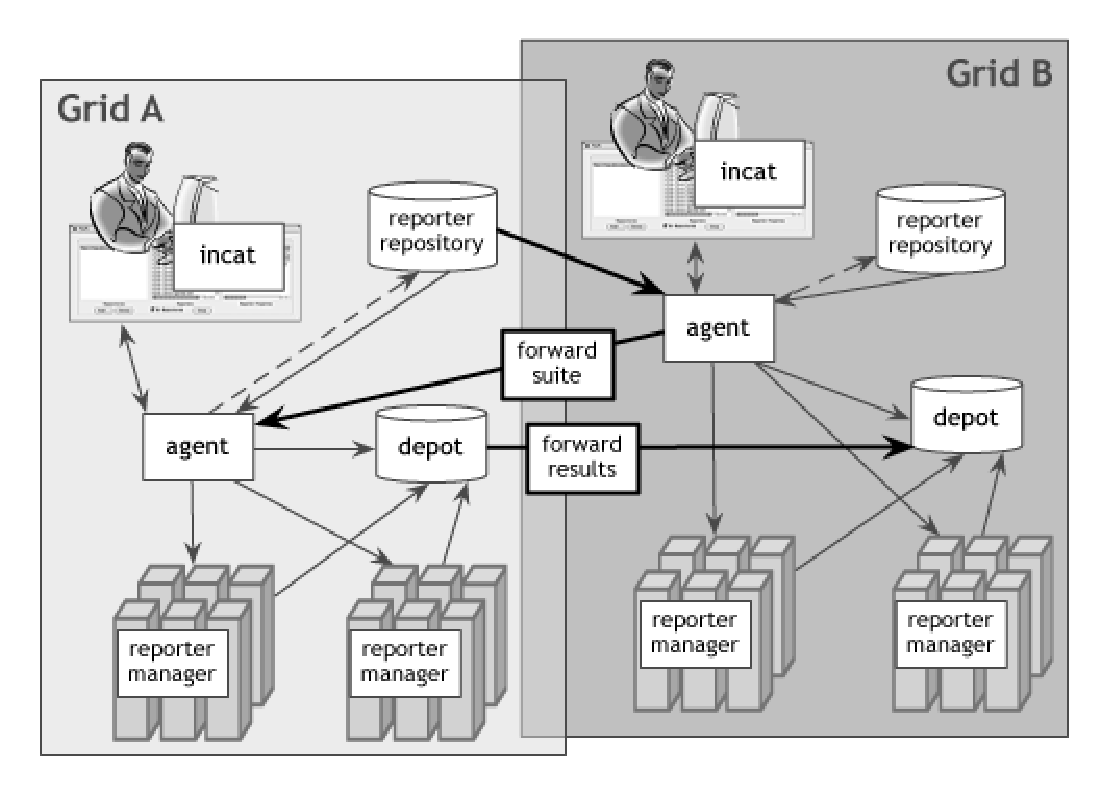
\includegraphics[width=.6\textwidth]{vo.eps}
  \caption{\label{tg_coord_fig} Coordinated Inca deployments.}
\end{figure*}

A planned extension to Inca 2 supports the distribution of control and storage
workload among multiple Inca components.  Figure~\ref{tg_coord_fig} shows a
scenario where two Inca deployments coordinate with each other.  This could
occur in application communities like GEON~\cite{geon}, which maintains its
own Grid but also has access to TeraGrid resources.   Running two Inca
deployments independently could result in duplicate testing.  Instead, we plan
to eliminate redundancy by allowing multiple deployments to coordinate suite
execution.
Figure~\ref{tg_coord_fig} shows this type of coordinated deployment, where Grid B 
has its own resources but also has access to resources in Grid A.
When an Inca administrator submits a suite to Grid B, the Inca agent running
on Grid B will determine which reporters run on Grid A resources and forward
them as a suite request to Grid A's agent.  If Grid B has permission to submit
suites, Grid A's agent will execute the suite and configure its depot to
forwards results back to Grid B's depot.  This extension is also expected
to provide the mechanisms for scalability and fault tolerance in the Inca
system.

%------------------------------------------------------------------------- 

\section{Use Cases}
\label{usecases}

\subsection{TeraGrid}

\begin{figure}[tbp]
  \centering
  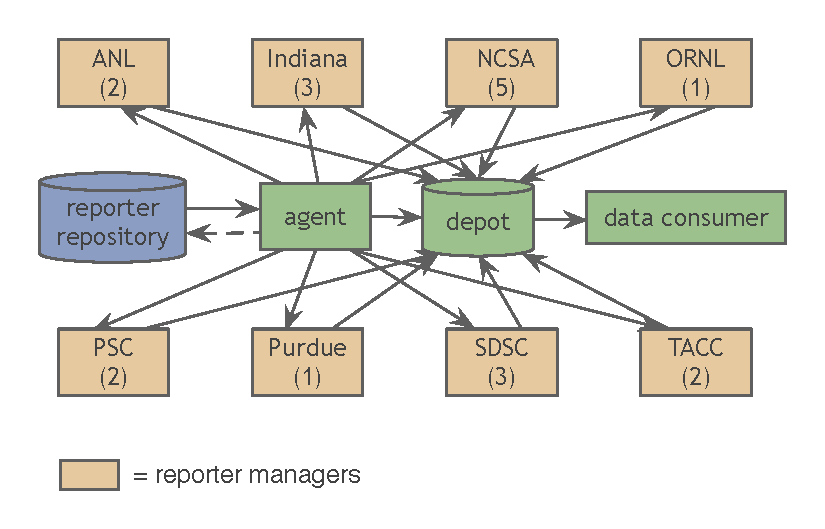
\includegraphics[width=.8\columnwidth]{tg-deploy.eps}
  \caption{\label{tg_deploy_fig} TeraGrid's Inca 2 Deployment.}
\end{figure}

\begin{figure*}[tbp]
  \centering
  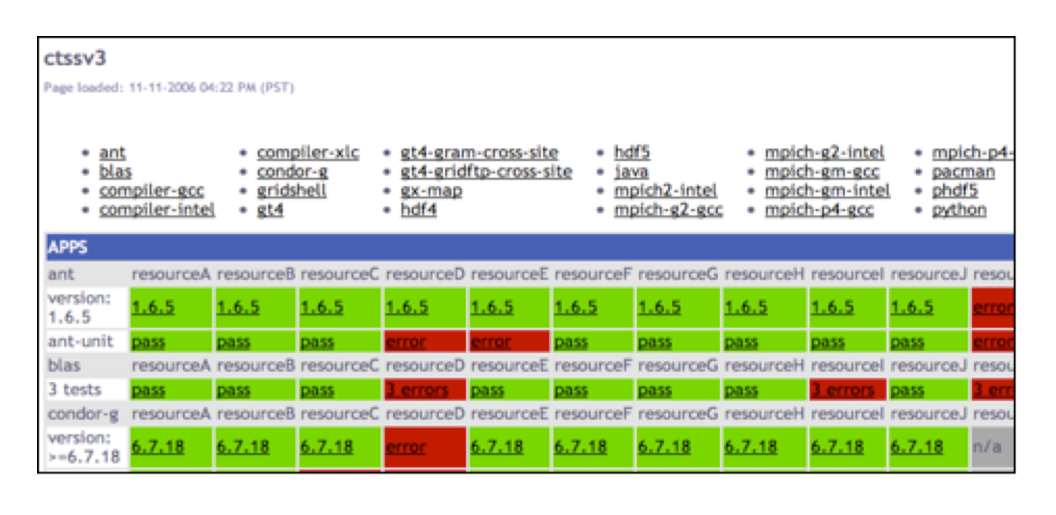
\includegraphics[width=.75\textwidth]{status-page.eps}
  \caption{\label{status_page_fig} Portion of the TeraGrid CTSSv3 detailed status page with the resources anonymized.}
\end{figure*}

% Description and Requirements - Describe CTSS
Requirements for user-level Grid monitoring on TeraGrid initially included the
validation and verification of Coordinated TeraGrid Software and Services (CTSS) 
on each TeraGrid resource.  As described in the introduction, CTSS was designed to
allow users to run Grid jobs more easily across its distributed, heterogeneous
resources.  CTSS version 3 (CTSSv3) is available on all TeraGrid compute
resources and contains approximately 30 software packages that provide
Grid tools and services (e.g., Globus, GSI-SSH, MyProxy), data management
tools (e.g., SRB, HDF5), and applications tools (e.g., MPICH, GCC).

To provide user-level monitoring of CTSS, Inca 1 was deployed on TeraGrid in
2003; TeraGrid's transition to Inca 2 completed in
November 2006.  In addition to CTSSv3 monitoring, Inca is now also being used
to collect job usage information from Globus 2 GRAM logs and to detect expired
host and CA certificates and CA CRLs. 

% Usage of Inca - Describe reporters, configuration, and deployment.  Figure.
A number of version and unit test reporters were developed to test the software packages in CTSS.
Currently, there are 56 such reporters executing an average of 109 series on
each of TeraGrid's 18 resources.  They include 48 all-to-all tests (GSI-SSH,
GRAM, and GridFTP), 20 Grid-related tests, 28 data-related tests, 30
application tool-related tests, and 2 security-related tests.  

The TeraGrid
Inca configuration makes extensive use of macros and resource groups and
currently uses 80 series and 82 resource macros to manage the total of 1,928
series executing on TeraGrid resources.
Figure~\ref{tg_deploy_fig}(a) illustrates TeraGrid's Inca 2 deployment
configuration.  The
agent, depot and consumer components are hosted at SDSC on 
sapa.sdsc.edu.  A reporter repository for TeraGrid is hosted
at SDSC on inca.sdsc.edu.  

% Results - Consumer view of CTSS, security, etc.
TeraGrid currently has six status pages to display the Inca monitoring
information: a summary of CTSSv3 test failures, a detailed grid of CTSSv3 test
results, a page showing grid job
usage, results for security tests, results for secure MDS tests, and a list of
all running reporters.

Figure~\ref{status_page_fig}(b) shows a portion of the TeraGrid detailed grid of
CTSSv3 test results
page.  CTSSv3 software packages are listed along the column and TeraGrid
resources (anonymized) in the header rows.  Test results for each package and
resource are shown in the table body rows.

\subsection{GrASP}
\label{grasp}

% Describe GrASP probes
The Grid Assessment Probes (GrASP)~\cite{grasp} are designed to 
serve as simple grid application kernel exemplars as well as a 
set of diagnostic tools. They test and measure the performance of 
basic Grid functions including file transfers, remote execution, 
and information services queries.  There are two basic probes: circle and 
gather.  The circle probe transfers a 100 MB file around a ring of
Grid nodes and measures the transfer time at each step.  The gather probe
transfers a 100 MB file from some number of source nodes to a compute node,
runs a computation through the job queue on the compute resource, and then
transfers a 100 MB file to a single destination node.  The transfer of the
first set of files is executed in parallel.  Transfer, compute, and queue times are recorded.

The GrASP probes yield data about Grid infrastructure performance and reliability.
In order to be most useful, probe data must be gathered 
repeatedly over time and archived.
In addition to storing the performance measurements,
any error messages encountered must be stored as well.    
In order to
gather historical data, the GrASP probes were modified
to follow the Inca reporter specifications and deployed using Inca.
Porting the original code to follow the reporter specifications proved to be
trivial.  A number of scripts were then written to graph and analyze the GrASP
data and related error messages stored in the Inca depot.  

\begin{figure*}[tbp]
  \centering
  \mbox{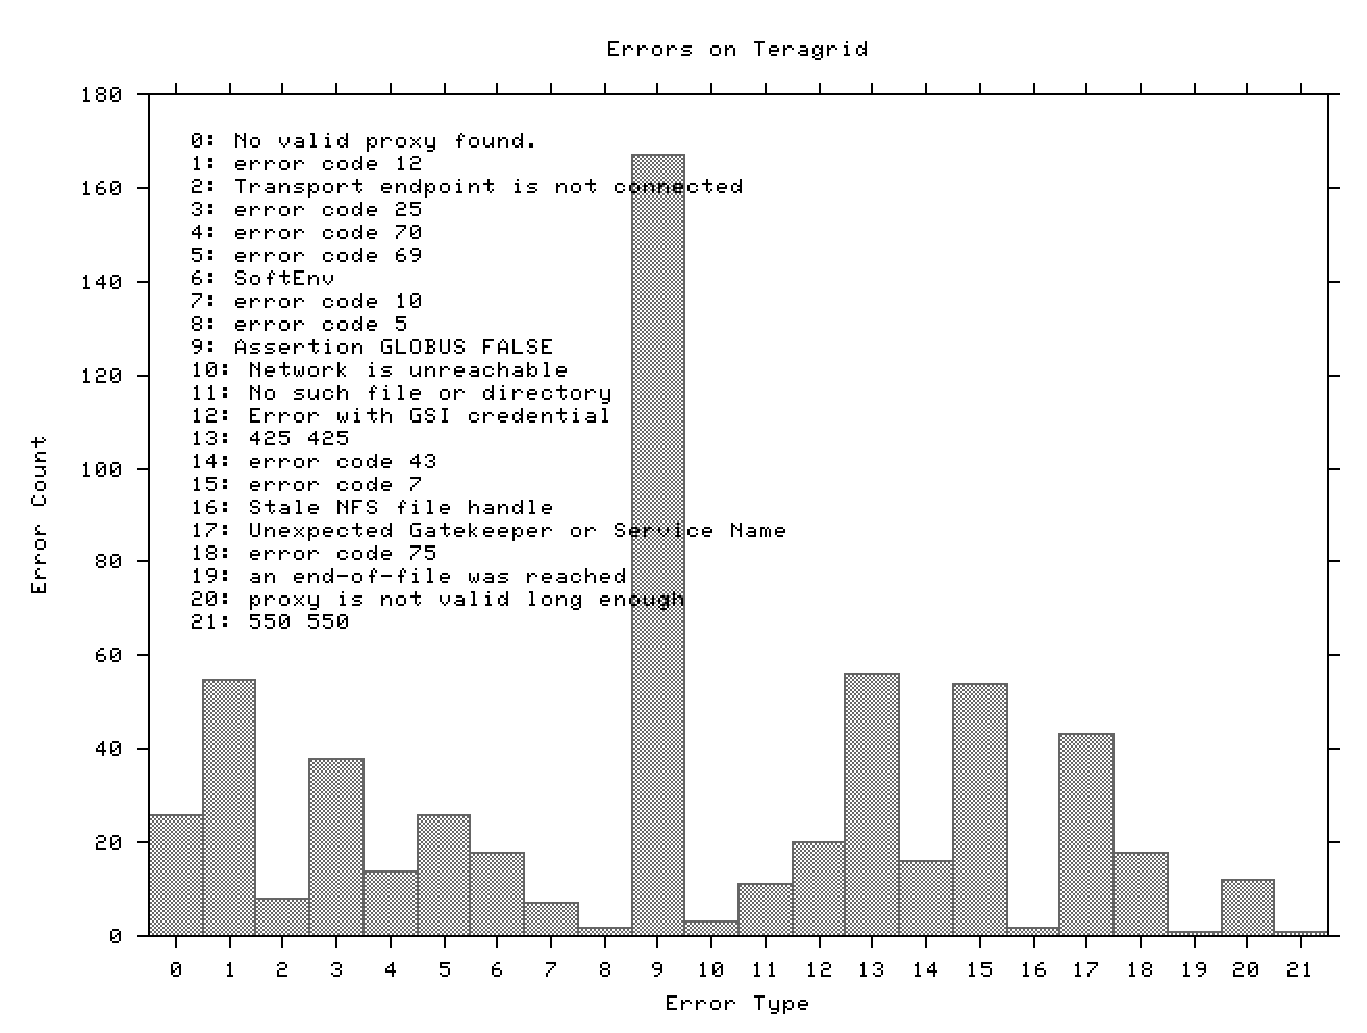
\epsfig{file=errorHistogramTG.eps, width=.6\textwidth}}
  \caption{\label{errorHist_fig} Number and types of errors collected by
  GrASP benchmark execution over a six-month period on TeraGrid.}
\end{figure*}

Using Inca, GrASP was deployed on TeraGrid and GEON for a period of over 6
months~\cite{grasp2}.  During this deployment, the execution time of Preco, 
a Grid application run on the TeraGrid, was predicted within 12\% (excluding setup and cleanup time).
A recurring Globus 2 bug was also identified as shown in Figure ~\ref{errorHist_fig}.  The figure shows the frequency and types (shortened) of 
system errors that were detected while executing 
GrASP on TeraGrid in 2005. The highest occurring
error was number 9, Assertion GLOBUS FALSE, which was the result of a bug in
the Globus 2 GRAM server.  

\subsection{Other Uses}

Other Inca users include the European DEISA Grid~\cite{deisa} and the UK National Grid
Service (NGS)~\cite{ngs}.  DEISA and NGS began using Inca in late 2004 and early 2005, respectively.  
Similar to TeraGrid, DEISA uses Inca to verify their Common
Production Environment (DCPE) across 11 heterogeneous resources.  They
currently have 40 version reporters to verify each of the packages included in
DCPE.  In addition, they have unit reporters for the DEISA Applications Test
Suite (DATS) to check basic operation of the C/C++/Fortran compilers, the MPI
library, some numerical libraries, OpenMP jobs, CORBA middleware, and a third
party application.  DEISA is currently using Inca 1 and will transition to
Inca 2 in the next few months.

NGS currently has Inca 2 deployed on four resources to verify their Grid services (on eight sites) and compilers.  They have wrapped the GITS~\cite{gits} tests using a new
API developed by the GITS developer.  The GITS reporters include 17 tests, 
such as small job submissions and data transfers, that verify Globus and GSI-SSH functionality.
NGS also has 12 tests for their compilers and
utilize 2 security reporters from the Inca repository.

%------------------------------------------------------------------------- 
\section{Future Work}

In order to improve problem detection and diagnosis for system administrators,
we plan to add graph rendering and statistical
analysis capabilities to the Inca data consumer.  This will improve troubleshooting capabilities by
allowing errors to be understood in a historical context.  It will also enable
summary displays analogous to those generated by Web page statistics packages
like Webalizer~\cite{webalizer} that provide a number of useful
statistics.  We expect to follow recommendations from TeraGrid and other Inca
users on the types of statistics and graphs that will be most useful.
Our plan is to offer a default set of statistics and graphs that can be used
directly and to provide the capability to add others.

Also to aid system administrator troubleshooting,
we plan to enhance Inca with a knowledge base that can be used to
discuss problems and suggest solutions.
The knowledge base will be populated by solutions provided by
system administrators and self-moderated to
improve quality.
This knowledge base could provide a vital resource
for system administrators and offer a forum for sharing
valuable experience and skills.   

Finally, we plan to improve the fault tolerance of Inca by enhancing the
reporter manager so that it caches reports locally if it is unable to
contact the depot or sends reports to a backup depot if one is available.
The agent will similarly be enhanced to cache configuration changes locally or
send configuration to a backup depot if one is available in case of a depot
failure.

%------------------------------------------------------------------------- 
\section{Summary}

%1.  Motivate and differentiate the Grid monitoring Inca does 2. Describe Inca
%2 design and its benefits 3. Illustrate that Inca 2 design is mature and
%being used in production by several Grids 4. Be different from Inca 1 paper
The goal of user-level Grid monitoring is to test and measure Grid
infrastructure from an impartial user perspective and detect problems before
users notice them.  Inca 2 implements such a user-level Grid monitoring system
and provides a number of new and improved features over our first version,
Inca 1.  The architecture and features of Inca 2 enable an Inca administrator
to easily write and deploy tests and performance measurements to Grid
resources and maintain them in a changing Grid environment.  The storage,
archiving, and querying capabilities also enable in-depth analysis of Grid
errors and performance in a historical context, which benefit Grid
operators and system administrators.  Inca 2 also provides a number of
security features such as short-term proxy management.
A production version of Inca 2 was released in February 2007 and
has been used in production environments to verify the common user environment
of TeraGrid and to execute and collect data for a set of Grid benchmarks on
both TeraGrid and GEON.  Future enhancements of Inca 2 will improve its fault
tolerance and enable more in-depth analysis of the overall Grid health and
behavior.  They will also make it easier to detect and resolve errors
and understand them in a historical context.  The features that Inca
provides and its proposed enhancements improve the stability of the
Grid infrastructure it monitors, ultimately improving the productivity of
scientists who conduct research on a Grid. 

%------------------------------------------------------------------------- 
\section{Acknowledgements}

The authors would like to thank Denis Girou and David Spence for providing
details for the DEISA and NGS Inca deployments, respectively.  This work was
supported by NSF grants SCI-0503944, SCI-0438741, and SCI-0503697.

%------------------------------------------------------------------------- 

\bibliographystyle{abbrv}
\begin{thebibliography}{10}

\bibitem{gridice}
S.~Andreozzi, N.~D. Bortoli, S.~Fantinel, A.~Ghiselli, G.~L. Rubini,
  G.~Tortone, and M.~C. Vistoli.
\newblock {GridICE: a monitoring service for Grid systems}.
\newblock {\em {Future Generation Computer Systems}}, 21(4):559--571, 2005.

\bibitem{grasp}
G.~Chun, H.~Dail, H.~Casanova, and A.~Snavely.
\newblock {Benchmark Probes for Grid Assessment}.
\newblock April 2004.

\bibitem{clumon}
{Clumon Web page}.
\newblock \url{http://clumon.ncsa.uiuc.edu}, 2007.

\bibitem{apt}
{Debian -- The Universal Operating System}.
\newblock \url{http://www.debian.org}, 2007.

\bibitem{deisa}
{Deisa - Distributed European Infrastructure for Supercomputing Appications}.
\newblock \url{http://www.deisa.eu/}, 2007.

\bibitem{globus}
I.~Foster and C.~Kesselman.
\newblock {Globus: A Metacomputing Infrastructure Toolkit}.
\newblock {\em International Journal of Supercomputer Applications},
  11(2):115--128, 1997.

\bibitem{hibernate}
{Hibernate Web page}.
\newblock \url{http://www.hibernate.org}, 2007.

\bibitem{jetty}
{Jetty Web page}.
\newblock \url{http://jetty.mortbay.org}, 2007.

\bibitem{grasp2}
O.~Khalili, J.~He, C.~Olschanowsky, A.~Snavely, and H.~Casanova.
\newblock {Measuring the Performance and Reliability of Production
  Computational Grids}.
\newblock September 2006.

\bibitem{monalisa}
I.~Legrand, H.~Newman, R.~Voicu, C.~Cirstoiu, C.~Grigoras, M.~Toarta, and
  C.~Dobre.
\newblock {MonALISA: An Agent based, Dynamic Service System to Monitor, Control
  and Optimize Grid based Applications}.
\newblock In {\em CHEP 2004}, Interlaken, Switzerland, September 2004.

\bibitem{log4j}
{Log4J Project Web page}.
\newblock \url{http://logging.apache.org/log4j}, 2007.

\bibitem{ganglia}
M.~Massie, B.~Chun, and D.~Culler.
\newblock { The Ganglia Distributed Monitoring System: Design, Implementation,
  and Experience}.
\newblock {\em Parallel Computing}, April 2004.

\bibitem{mom}
{Microsoft Operations Manager}.
\newblock \url{http://www.microsoft.com/mom}, 2007.

\bibitem{myproxy}
{MyProxy Credential Management Service}.
\newblock \url{http://myproxy.ncsa.uiuc.edu}, 2007.

\bibitem{ngs}
{NGS Web page}.
\newblock \url{http://www.grid-support.ac.uk}, 2007.

\bibitem{ncsa-test}
{NCSA TestGrid Project}.
\newblock \url{http://grid.ncsa.uiuc.edu/test}, 2007.

\bibitem{nagios}
{Nagios Web page}.
\newblock \url{http://www.nagios.org}, 2007.

\bibitem{geon}
A.~K. Sinha, B.~Ludaescher, B.~Brodaric, C.~Baru, D.~Seber, A.~Snoke, and
  C.~Barnes.
\newblock { GEON: Developing the Cyberinfrastructure for the Earth Sciences - A
  Workshop Report on Intrusive Igneous Rocks, Wilson Cycle and Concept Spaces}.
\newblock {\em Submitted to GSA Today}.

\bibitem{inca1}
S.~Smallen, C.~Olschanowsky, K.~Ericson, P.~Beckman, and J.~M. Schopf.
\newblock {The Inca Test Harness and Reporting Framework}.
\newblock In {\em Proceedings of Supercomputing 04}, November 2004.

\bibitem{teragrid}
{The TeraGrid Project Web page}.
\newblock \url{http://www.teragrid.org}, 2007.

\vfill\eject

\bibitem{tivoli}
{IBM Tivoli Monitoring Web page}.
\newblock \url{http://www.ibm.com/software/tivoli/products/monitor/}, 2007.

\bibitem{gits}
{The UK Grid Integration Test Script - GITS}.
\newblock \url{http://www.soton.ac.uk/~djb1/gits.html}, 2007.

\bibitem{webalizer}
{Webalizer Web page}.
\newblock \url{http://www.mrunix.net/webalizer/}, 2007.

\end{thebibliography}

\end{document}


